\documentclass[a4paper, 11pt]{article}
\usepackage[margin=0.75in]{geometry}
\usepackage{amsmath}
\usepackage{graphicx}
\usepackage{natbib}
\usepackage{enumitem}
\usepackage{longtable}


% % line numbers
% \usepackage[left]{lineno}

% \usepackage[
% backend=biber,
% style=numeric,
% sorting=none
% ]{biblatex}
% \addbibresource{behavior.bib}

% \makeatletter
% \renewcommand{\@biblabel}[1]{\quad#1.}
% \makeatother

\usepackage{nameref,hyperref}

\begin{document}
\noindent {\LARGE \textbf{What is behavior? No seriously, what is it?}}

\vspace{6pt}\noindent {\large Adam Calhoun$^{1,*}$, Ahmed El Hady $^{1,*}$}

\vspace{6pt}

\noindent{\small $1$. Princeton Neuroscience Institute, Princeton University, Princeton, United States. 


\noindent * correspondence should be addressed to Ahmed El Hady(ahady@princeton.edu) or Adam Calhoun (adamjc@princeton.edu)}


\vspace{18pt}

\section*{Abstract}

Studying "behavior" lies at the heart of many disciplines. Nevertheless, a academics who study behavior rarely provide an explicit definition of what `behavior' actually is. What range of definitions do people use, and how does that vary across disciplines? To answer these questions we have developed a survey to probe what constitutes `behavior'. We find that academics adopt different definitions of behavior according to their academic discipline, animal model that they work with, and level of academic seniority. Using hierarchical clustering, we identify at least six distinct types of `behavior' which are used in seven distinct operational archetypes of 'behavior'. Individual respondents have clear consistent definitions of behavior, but these definitions are not consistent across the population. Our study is a call to action for academics to clarify what they mean by "behavior" whereever they study it, with the hope that this will foster interdisciplinary studies of behavior to improve our understanding of behavioral phenomena.

\vspace{18pt}
\section*{Introduction}

The scientific definition of `behavior' has tended toward the maxim `I know it when I see it'. But does everyone know and see the same thing? Much ink has been spilled coming up with precise definitions of behavior, stretching from Aristotle \cite{aristotle} to the present passing though Wiener's cybernetics \cite{wiener2019cybernetics}, Von Neumann \cite{von2012computer}, Lorenzian ethology \cite{lorenz2013foundations}, Tinbergen behavioral theory \cite{tinbergen1972animal} and Von Uekuell's umwelt \cite{uexkull1921umwelt}. Within the subfield of behavioral biology, Levitis et al  \cite{levitis2009behavioural} surveyed the literature and found 25 distinct operational definitions of behavior. These range from the vague (`what an animal does', \cite{davis1966integral}) to the specific (`‘A response to external and internal stimuli, following integration of sensory, neural, endocrine, and effector components. To date, there are no surveys that cover a wide variety of academic fields when it come to the definition of behavior.  More recent work has used operationalized definitions to create machine learning algorithms capable of `recognizing' when an animal is performing some `behavior' \cite{berman2014mapping,wiltschko2015mapping,calhoun2019unsupervised}.

% I think this needs a bit of editing but can be good
In the wake of technological advancements in machine learning, behavior can now be studied on increasingly finer scale. Naturally, this led to behavior being broken up into distinct classes. For instance, sensorimotor behavior is behavior that relates sensory input to motor output. But is this `behavior' when it is performed by a rat? How about a C. elegans, with only three or four synapses between sensory neurons and motor output? What about a bacteria or a computer program? Furthermore, during this behavior not only is the animal moving but there are cognitive variables and needs that influence the animal's action. Which of these constitute the `behavior'? As scholars cross disciplinary boundaries and increasingly perform statistical and scientific work on behavior, clarity as to what is being worked on is vital. We should know if when an economist explains `behavior' and a neuroscientist explains `behavior' whether they are referring at all to the same thing. The contrast between neuroeconomics and behavioural economics exemplifies this. While in neuroeconomics, researchers uses tools from neuroscience to study how a subject's brain perform economical computations, behavioural economics is concerned with studying biases and heuristics that subjects employ while performing real world decisions . Same contrast can be found in other sub-fields of neuroscience, systems neuroscientists seek to understand neural mechanisms of behavior, cognitive scientists seek to understand cognitive mechanisms underlying it. On the other hand, behavioural ecologists seek to study how behavior is shaped by the environment, while sociologists seek to understand society through the behavior of its individuals. If someone said they understood the neural basis of behavior, do they mean the ability to produce a motor output? The ability to mentally compare to objects? The mentally compare two objects and act on it?

Instead of creating our own definition of behavior, we aimed to identify how the word `behavior' is actually used by the academic community.We designed a survey aimed at this question. Through a quantitative analysis of survey data, we show that what constitutes `behavior' differs between academic disciplines, level of academic seniority, and type of animal model organism studied. We further show that there are at least six `types' of behavior that are used to construct eight definitions of behaviors. 

The study pinpoints to the lack of a common inter-disciplinary definition of behavior. We argue that we do not need an agreed-upon singular definition of behavior, but we do have to be clear on what the definitions that we are using are in any given study. Those clear working definitions will open up the opportunity for effective interdisciplinary studies that tackle multiple facets of "behavior"

\vspace{24pt}
\section*{Results}

\subsection*{Widespread disagreement of definitions of behavior}
We sought to clarify how the term `behavior' is being used. In order to answer this, we developed a set of questions designed to probe different aspects of 'behavior'. For instance, 'A behavior is always the output of motor activity', 'Is learning a behavior?', and 'Is a dog that follows a scent trail behaving?'. We included questions that were designed to elicit inconsistencies such as, 'Is a reflex a behavior?' and 'Is sweating a behavior?'. The order of questions was randomized and the survey was distributed online and elicited responses from a range of academic disciplines and seniorities (see Methods, Table 1 and 2). Analysis revealed that respondents did not provide a consistent answer for the the majority of questions: 43 / 48 answers had less than 80\% of respondents answering in the same manner (Table 1, Supplemental Fig 1a). While there were some questions that showed widespread agreement in either a `Yes' ('Is a dog that follows a scent trail behaving') or a `No' ('Does a behavior need to be intentional') answer (Supplemental Fig 1b-d), most questions showed disagreement. The questions with the most disagreement (defined as the highest uncertainty, or entropy, in their responses), included 'Can computer programs behave?' and 'A behavior always involves interaction with the environment?' (Fig 1a).

A previous survey of professionals in animal behavior\cite{levitis2009behavioural} had observed that respondents were inconsistent and self-contradictory. Was this true for our survey? We used a regression model to ask whether we could predict responses from the answers to previous questions and found that we could (Fig 1b). This was true both on average and across all questions (accuracy X\% +/- Y \%). This suggests that disagreement on behavioral questions represents disagreement on the underlying definition of behavior itself.

We then asked whether this variation in responses could be due to differences in academic disciplines - perhaps those trained in the Humanities would have a fundamentally different idea of 'behavior' from those trained in Engineering, for instance. We embedded responses in a lower-dimensional space using multiple correspondence analysis (MCA), a factor analysis technique for categorical variables \cite{le2010multiple} (Supp Fig 2). For visualization purposes, we grouped subjects into broad categories academic categories: Biological Sciences, Math/Engineering, Ecology, and Humanities (see Methods for definitions, but see Supplemental Fig 3 for all disciplines). We found differences between each field (Fig 1c, Supp Fig 3a, 4a). We  hypothesized that even within a field there might be substantial differences; a Cognitive Neuroscientist gets different training from a Systems Neuroscientist. Again, plotting the mean responses for each sub-field showed significant differences (Fig 1d, Supp Fig 4b).

In behavioral research, scientists can ask fundamentally different questions about behavior when they work with humans than when they work with invertebrates. For instance, C. elegans researchers typically investigate chemotaxis and thermotaxis, which are activities that involve sensorimotor transformations, while researchers who study humans may be more likely to study cognitive activities like abstract decision-making. Additionally, in neuroscience those who study invertebrates can map behavior to a single-neuron level, something not typically done in mice or humans.  We thus divided subjects by the model organism that they work with. We again find differences between model organisms (Fig 1e, Supp Fig 3b,4c). Surprisingly, we also found that academic experience is also associated with differences in behavioral definitions (Fig 1f, Supp Fig 4d).

\begin{figure}
\centerline{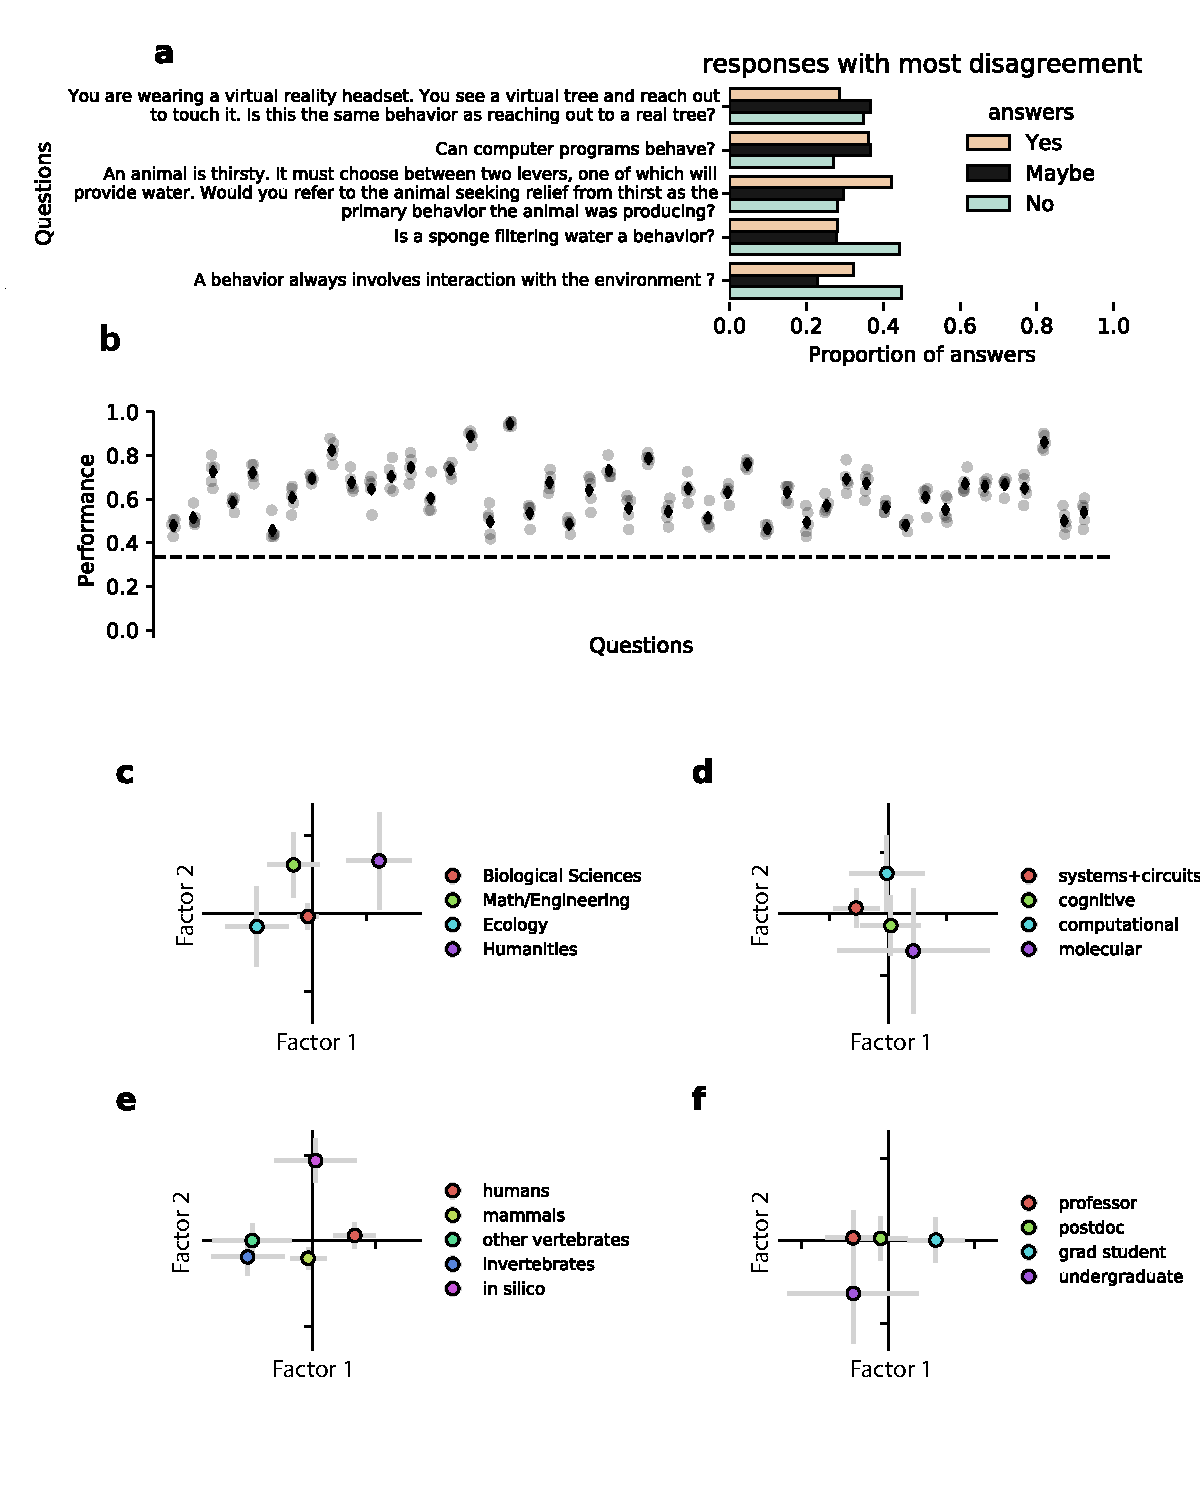
\includegraphics[width=\textwidth]{fig1.pdf}}
\caption{Definitions of behavior are varied but internally consistent} \textbf{a}, The five questions with the most disagreement between respondents as defined by the response entropy (n=455). \textbf{b}, Responses are predictable with a regression model. Gray dots represent the performance at predicting answers on held-out data using 5-fold cross-validation, black diamond is mean. The dashed line represents chance performance. \textbf{c-f}, We used a factor analysis (Multiple Correspondence Analysis (MCA)) to reveal how groups responded on similar questions. Plotting responses on the two largest factors, colored by (\textbf{d}) scientific field, (\textbf{e}) neuroscience specialty, (\textbf{f}) model organism used, and (\textbf{g}) academic seniority. All data shown is the mean, and error bars are SEM.
\end{figure}

\subsection*{Hierarchical clustering finds definitions}

One possibility is that these differences between fields are not because each has a different definition of behavior, but because certain behavioral definitions are more common in that field. In order to identify potential definitions of behavior, we performed hierarchical clustering on both the responses and respondents (Fig 2). We found six potential classes of questions and seven potential classes of responses. 

For each respondent cluster - which we call a 'behavioral archetype', answers were relatively consistent in each behavior-type cluster. In order to gain insight into what each behavioral archetype corresponds to, we examined the mean rate  of 'Yes' responses within each behavior-type/definition cluster (Fig 3a). In the first behavioral definition cluster (related to 'reflexes') the mean response was 67\% Yes, but this showed large variability within definition clusters. For instance, the A definition had 94\% of all responses as 'Yes' while the D and G clusters had 19\% and 25\% of responses as Yes, respectively. To better understand this, we plotted the change in responses relative to the overall mean for 'Yes', 'No', and 'Maybe' responses (Fig 3b-d, Supp Fig 3a-b). We note that different definition clusters show large differences in which answer changes by Definition cluster; behavior-type B shows only negligible differences in Yes responses, while it shows changes in No or Maybe responses whereas behavior-type C shows very little change in No responses but many changes in Yes responses.

\begin{figure}
\centerline{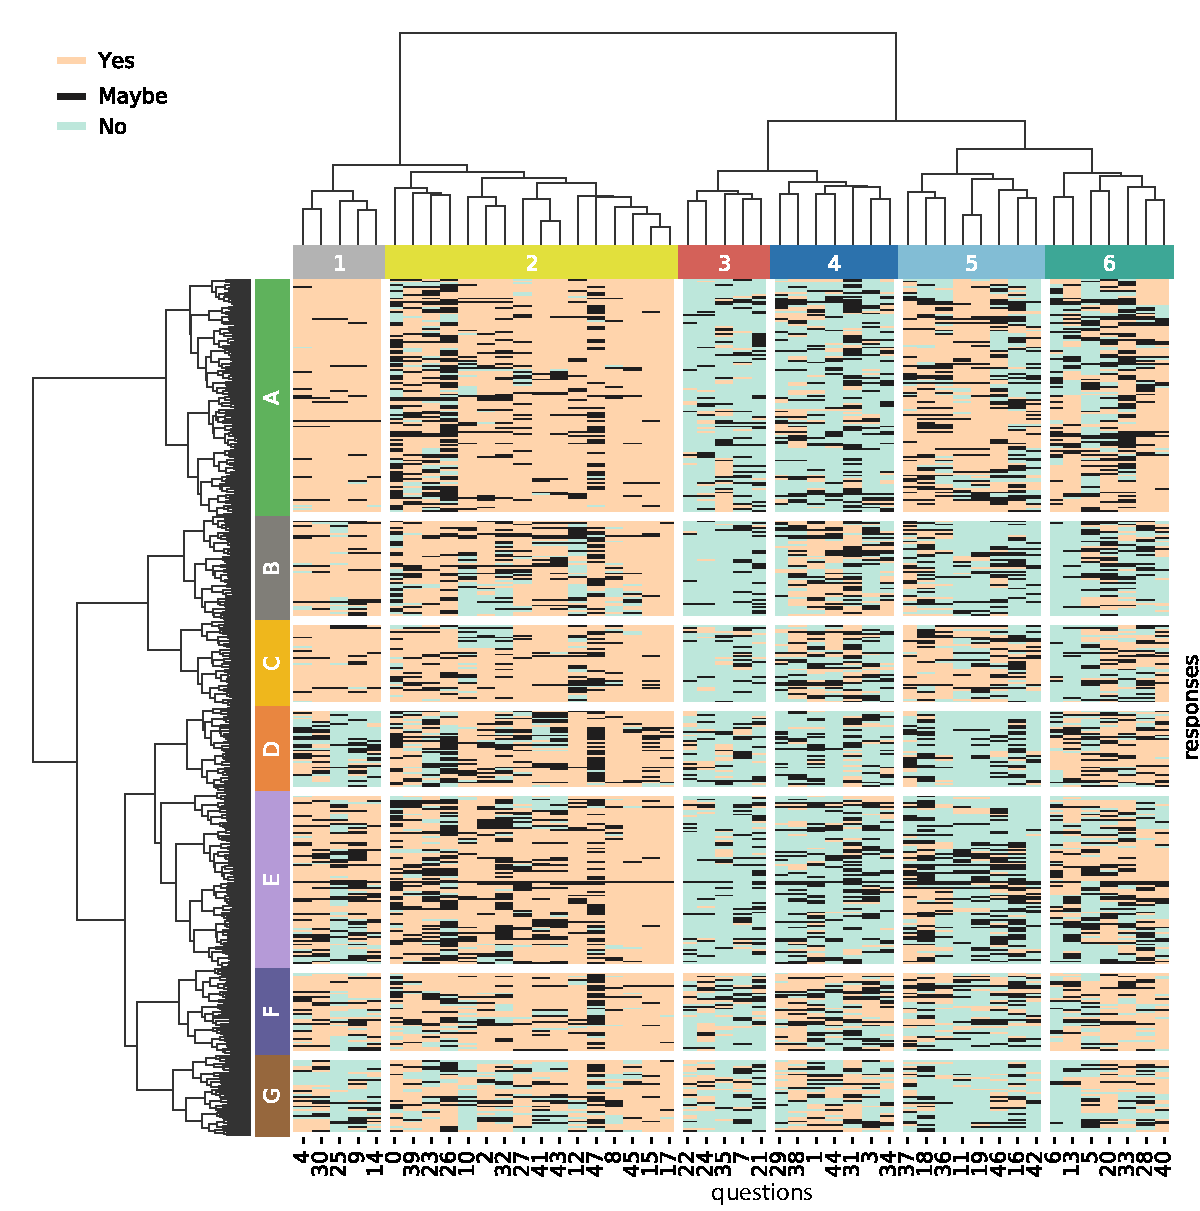
\includegraphics[width=\textwidth]{fig2.pdf}}
\caption{Survey responses reveal clustered definitions of behavior.} Hierarchical clustering on the 455 responses reveals six categories of questions and seven categories of responses. The six categories of questions, labeled 1-6, are particular types of behavior, and the seven categories of responses, labeled A-G, are behavioral definitions. See Figures 3 - 4.
\end{figure}


% \begin{enumerate}[label=\Alph*]
%     \item \textbf{broad} - Reflexes are behavior, everything behaves, no need for intentionality, behavior is not predominantly motor, non-animal behaviors, l\&m is behavior

%     \item \textbf{Motor outputs (animals only)} - Reflexes are behavior, everything behaves, no need for intentionality, behavior is predominantly motor, only animals behave, l\&m is not behavior

%     \item \textbf{Broad (but mostly motor)} - Reflexes are behavior, everything behaves, no need for intentionality, behavior is predominantly motor (mixed answers), non-animals behave, memory is not behavior and don't need to anthropomorphize but otherwise cognition is behavior [difference between this and A (broad) is that MUST be motor/sensormitor and less likely L&M/cognition)] [difference between this and B is relatively higher 5, a little 6]

%     \item \textbf{Cognition (and anthropomorphizable animal behaviors)} - Reflexes are not behavior, not clear if everything behaves, need to anthropomorize but otherwise no need for intentionality, behavior is not predominantly motor, no non-animal behaviors, learning and memory is behavior [note fewer YESes so this is a more 'specific' category]

%     \item \textbf{Broad (animals only)} - Reflexes are behavior except for the sucking reflex (babies), unclear about inferring cognition, not intentionality, no non-animal behaviors, [big difference between A and E is that non-animals, and non-cognitive things like babies, don't behave] [mostly defined by NOs - this is average for 1 and 2, and lower YESes for everything else] [difference from B is lower 4 and higher 6]

%     \item \textbf{Well-defined/understood animal behaviors} [difference between and F is lower 5 higher 4 and 3]

%     \item \textbf{Animals acting with intentions} - Reflexes are not behavior, but behavior is motor [YES to 2, relatively high 3 and 4, low 1 and 5]
% \end{enumerate}

Examining the questions in the response clusters revealed that similar questions were in each cluster (Table 3, Fig 3). For instance, Cluster 1 was filled with questions about whether reflexes count as behaviors ('Is a baby urinating a behavior?', 'Is a reflex a behavior?', 'Is the sucking reflex a behavior?', and so on). Based on this, we term these 'behavior definition clusters' and labeled them as:

\begin{enumerate}
 \item Reflex (Fig 3a)
 \item Actions (Fig 3b)
 \item Understanding the mind  (Fig 3c)
 \item Motor or sensorimotor  (Fig 3d)
 \item Non-animal  (Fig 3e)
 \item Cognition  (Fig 3f)
\end{enumerate}

\begin{figure}
\centerline{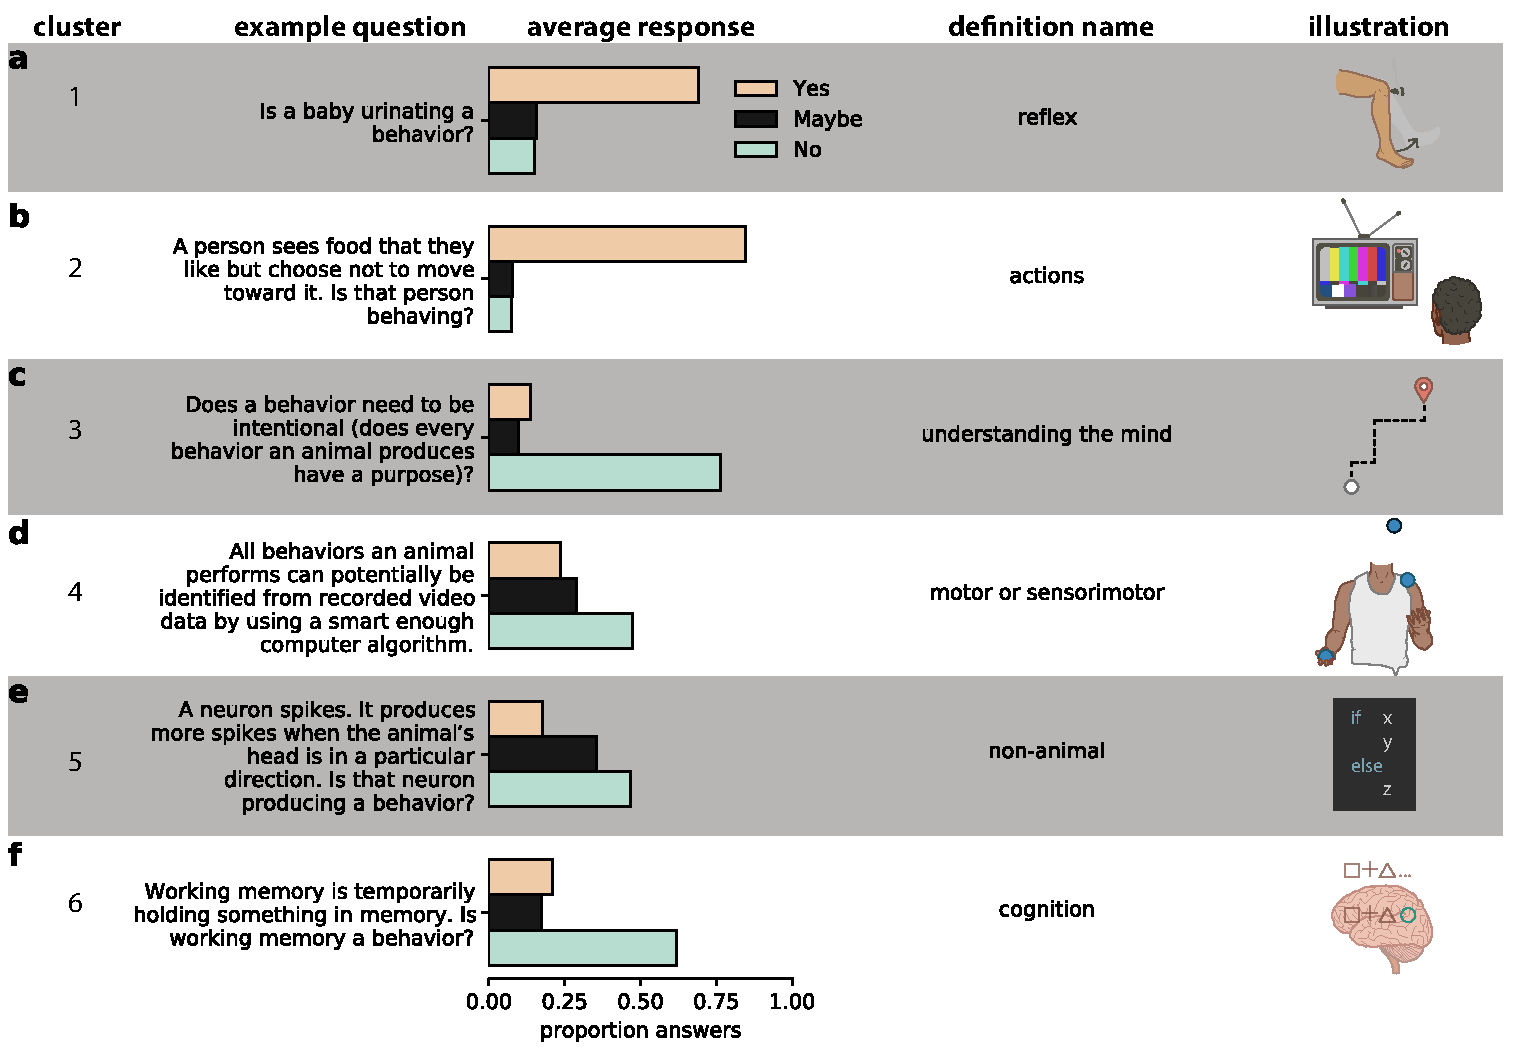
\includegraphics[width=\textwidth]{fig3.pdf}}
\caption{Behavioral archetypes revealed by clustering.} \textbf{a-f}, Example questions for each type of behavior (left). Illustration representing that type of behavior (right). These definitions are (a) Reflex, (b) actions are behavior, (c) we must understand the mind of an animal to identify its behavior, (d) motor or sensorimotor, (e) non-animal behaviors, (f) learning and memory/cognition.
\end{figure}

\subsection*{Behavioral archetypes}

For each respondent cluster - which we call a 'behavioral archetype', answers were relatively consistent in each behavior-type cluster. In order to gain insight into what each behavioral archetype corresponds to, we examined the mean rate  of `Yes' responses within each behavior-type/definition cluster (Fig 4a, Supplemental Fig 5). In the first behavioral definition cluster (related to `reflexes') the mean response was 67\% Yes, but this showed large variability within definition clusters. For instance, the A definition had 94\% of all responses as `Yes' while the D and G clusters had 19\% and 25\% of responses as Yes, respectively. To better understand this, we plotted the change in responses relative to the overall mean for `Yes', `No', and `Maybe' responses (Fig 4b, Supp Fig 6). We note that different definition clusters show large differences in which answer changes by Definition cluster; behavior-type B shows only negligible differences in `Yes' responses, while it shows changes in `No' or `Maybe' responses whereas behavior definition C shows very little change in `No' responses but many changes in `Yes' responses.

Based on these, we named these archetypes by examining which behavioral definitions were being used:

  \begin{enumerate}[label=\Alph*]
    \item Broad
    
    \item Motor outputs (animals only)

    \item Broad (but mostly motor)

    \item Cognition (and anthropomorphizable animal behaviors)
    
    \item Broad (animals only)
    
    \item Well-defined/understood animal behaviors

    \item Animals acting with intentions
\end{enumerate}

Taking this all together, we show how behavioral archetypes are made up of different behavioral definitions (Fig 4c).

\begin{figure}
\centerline{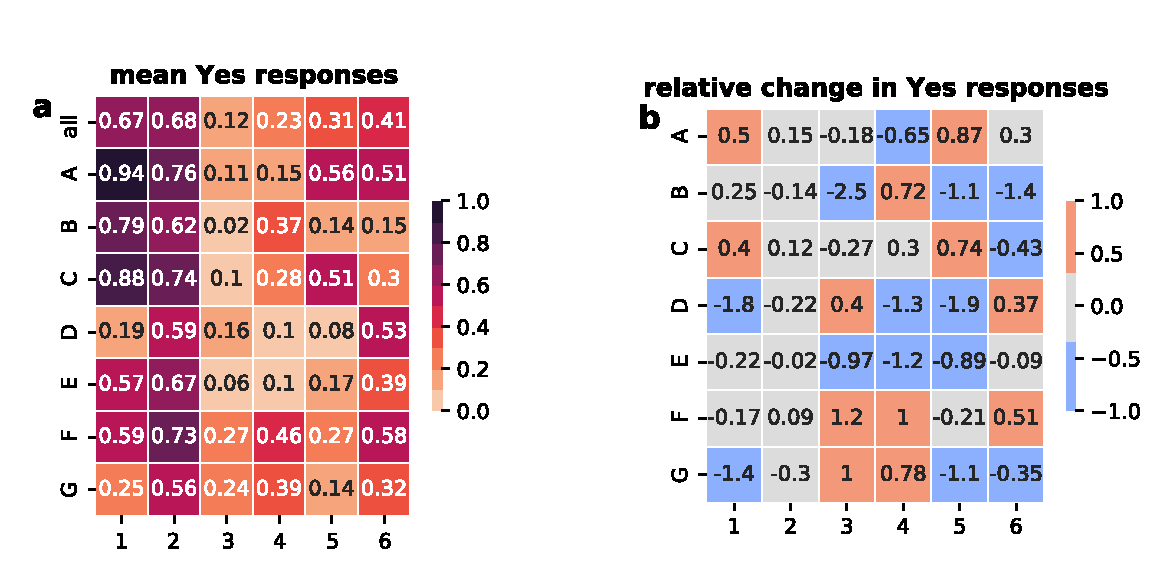
\includegraphics[width=\textwidth]{fig4.pdf}}
\caption{Validation and consistency of behavioral archetypes} \textbf{a} Responses are consistent (regression). \textbf{b}, The mean `Yes' response in each category allow us to understand what the definitions are composed of. \textbf{c}, Kathleen's illustration: behavior definitions and types
\end{figure}
% Change in 'Yes' response relative to all data show key differences to each question category. Values plotted are the 2-fold change in response relative to overall mean, coded so that blue is $<$ -0.33, red is $>$ 0.33 and grey is in between. \textbf{d-e}, Same as \textbf{b}, but for Maybe and No responses, respectively.

\subsection*{Academic fields use different archetypes}
% what happens when we look at the behavioral definitions/types??
We next used these behavioral archetypes to ask whether different academic fields are consistently using different archetypes when they refer to `behavior'. Respondents who come from the humanities were dramatically less likely to be part of the `broad' (A) archetype and much more likely to be a part of the `acting with intentions' (G) archetype. Ecologists were relatively more likely to be part of the `broad (mostly motor)' (C) and `broad (animals only)' (E) archetypes. Within neuroscience specialties, molecular neuroscientists were more likely to be a part of the `broad (mostly motor)' (C) archetype and cognitive to be part of the `well-defined/understood behaviors' (F) archetype. The `broad (animals only)' (E) archetype was almost entirely Systems and Computational neuroscientists.

When broken down by the organism used for the work, those who worked with Humans were the least likely to use `broad' (A) and `broad (animals only)' (E) archetypes but the most likely to use the `cognition' (D) and `well-defined/understood behaviors' (F) definitions. `Other vertebrates' dominated `broad' (A) and `broad (animals only)' (E) and invertebrates were 50\% more likely to be a part of `broad (but mostly motor' (C).

Undergraduates were predominantly a part of archetypes `broad' (A) and `acting with intentions' (G), whereas professors were the most likely to be part of cluster `motor outputs (animals only)' (B).

% this is figure 5
\begin{figure}
\centerline{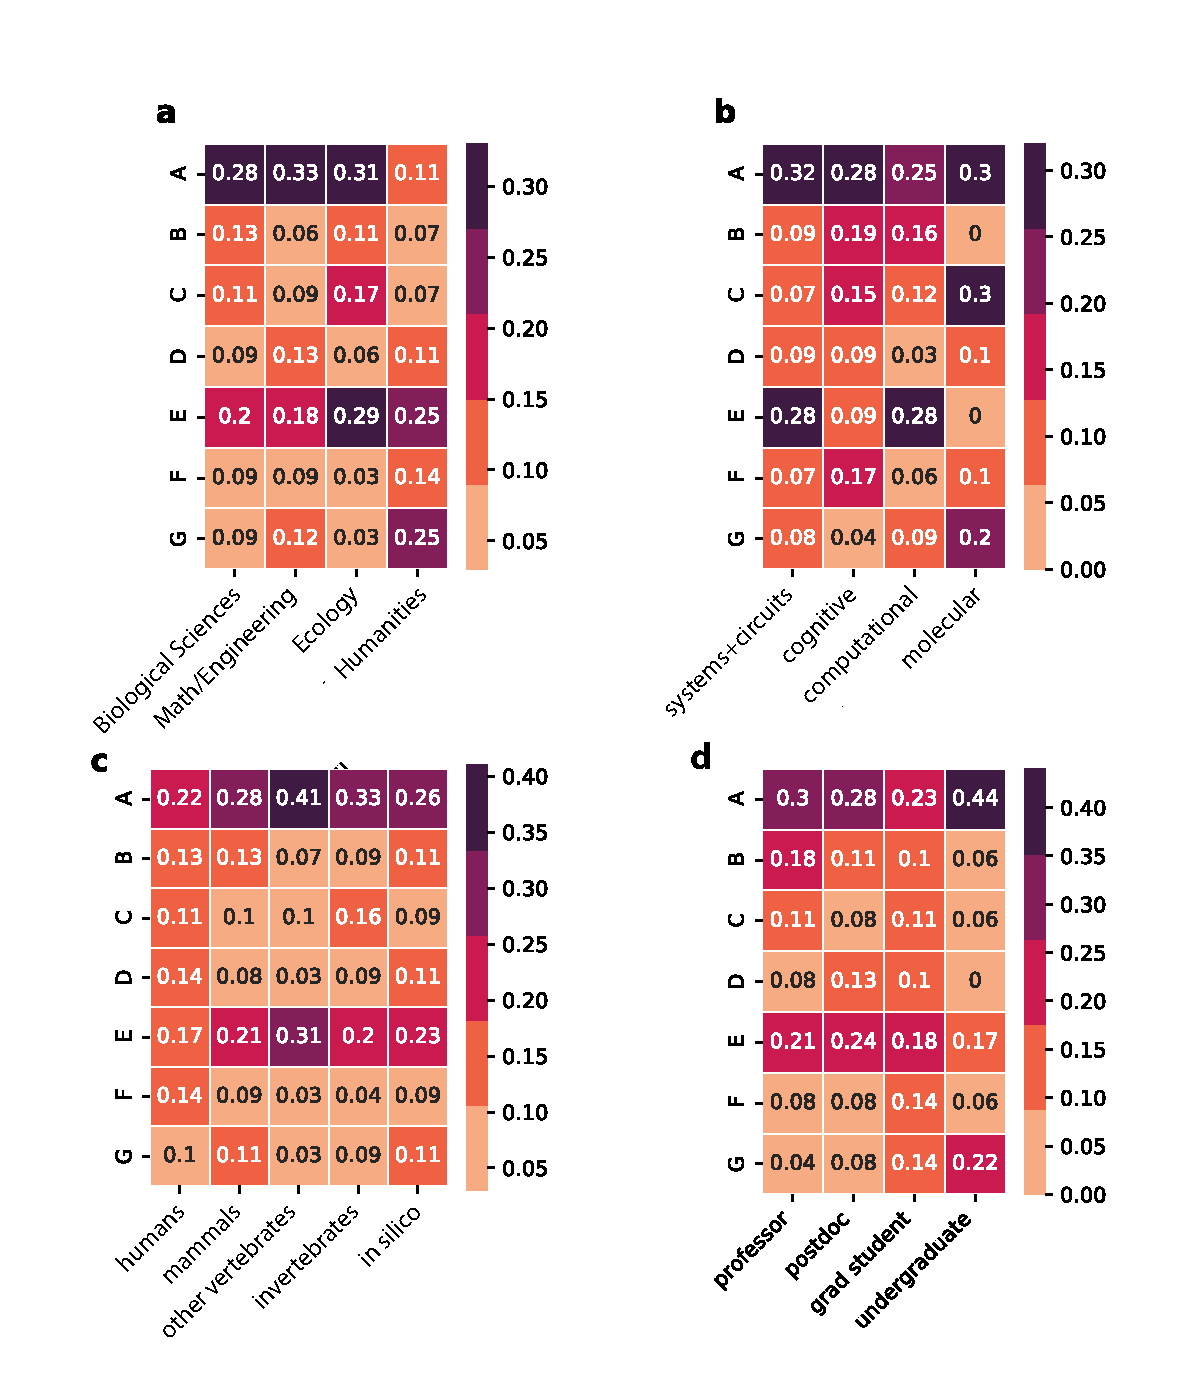
\includegraphics[width=\textwidth]{fig5.pdf}}
\caption{Different groups have distinct distribution of definitions.} \textbf{a}, Academic fields show different propensities to use each category of 'behavior'. This is also true of \textbf{b} neuroscience specialties, \textbf{c} model organism used, \textbf{d} and academic seniority. See Methods for definitions of each field.
\end{figure}

\subsection*{No commitment to behaviorism or cognitivism}
Behaviorism and Cognitivism are two main schools of thought regarding behavior. These constitute A, B, C. However, it is unclear if colloquial definitions of behavior actually relate to these definitions. In order to answer these questions, we assigned each of our survey questions to supporting behaviorism, supporting cognitivism, or being unrelated to either (see Methods). Individual responses were assigned a score from -1 to 1 relating to the number of ``Yes"es or ``No"s that were answered for the relevant questions (Fig 6a). We find that very few respondents are strongly Behaviorist or Cognitivist, on either an individual level (Fig 6a, histograms) or a group level. We further asked whether this was true of specific groups; we might expect, for instance, that those who are highly trained in behavior or cognitive psychology might tilt more strongly to one side or another. [REPORT RESULTS HERE; LOOK AT FACULTY VS GRAD STUDENTS AND THEN COGNITIVE PSYCHOLOGY VS SOME OTHER FIELD??].

% figure 6 - behaviorist/cognitivist
\begin{figure}
\centerline{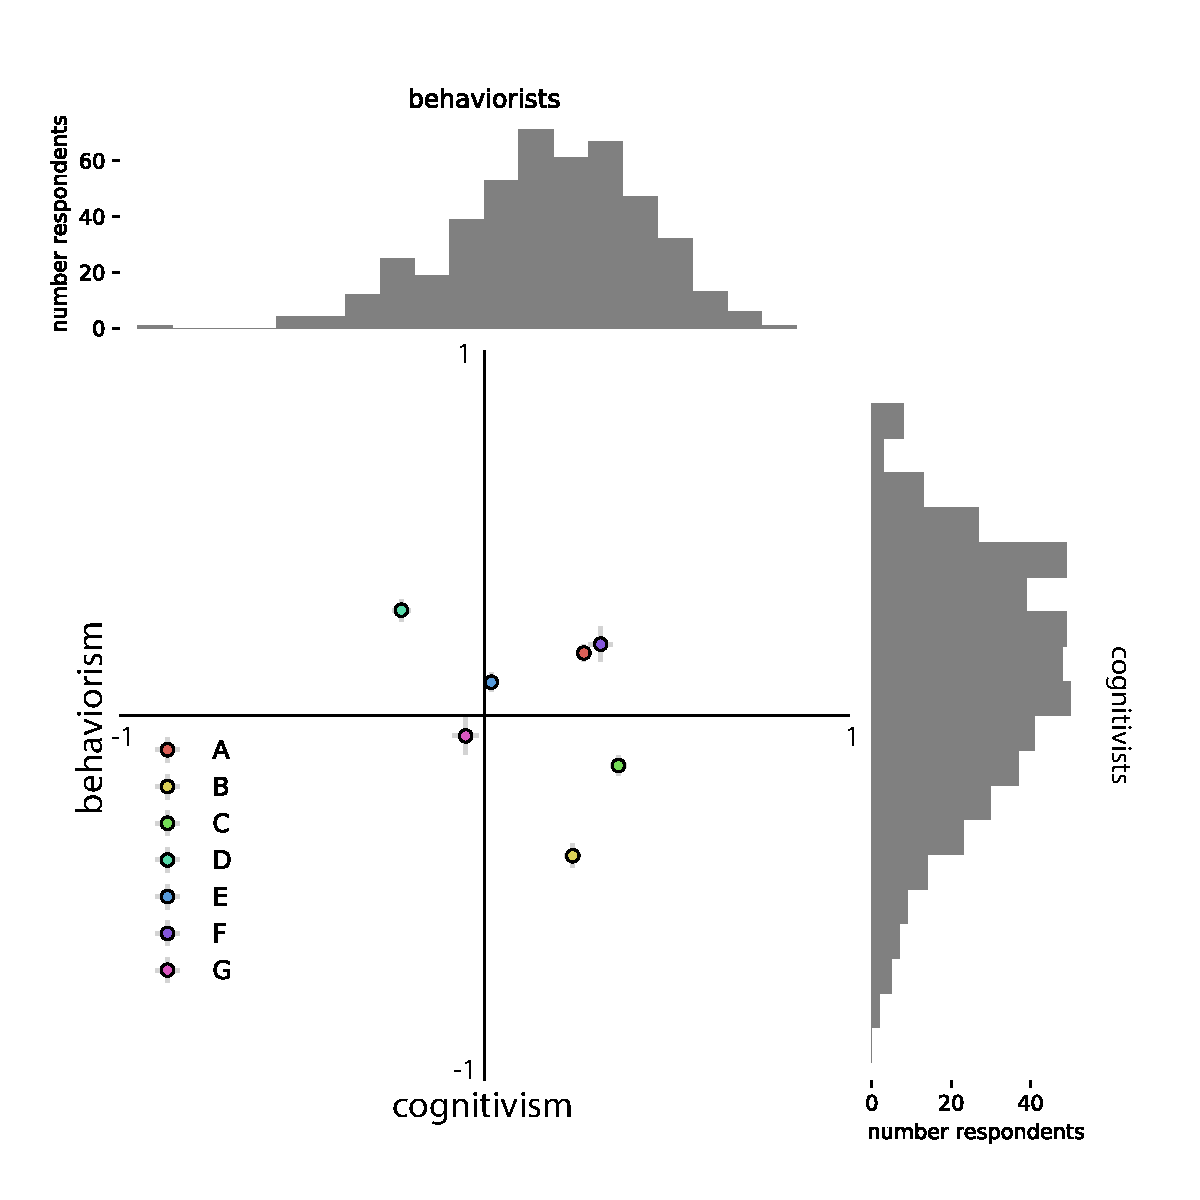
\includegraphics[width=\textwidth]{fig6.pdf}}
\caption{No one cares about behaviorism and cognitivism.} Questions were labeled 'behaviorist', 'cognitivist', or 'neither'. Responses were scored to either totally agree (+1) or totally disagree (-1) with each category. Respondents did not agree with behaviorism or cognitivism, but used definitions that were a mix of the two. Generally, though, the categories had a negative correlation between behaviorism and cognitivism. Circles represent mean and error bars are +/- SEM.
\end{figure}
% can try 

\section*{Discussion}

In this study, we have shown that `behavior' is not universally defined by academics. We have developed and analyzed a survey that has allowed us to identify how the term `behavior' is used, and what it means to people belonging to different academic communities. Using this survey, we have shown that important differences exist in what an academic community would consider to be `behavior', and additionally identified seven behavior-type clusters and six definition clusters. These behavioral archetypes correspond roughly to the following labels `broad', `animal motor outputs are behavior', `broad but motor', `animal+cognitive', `animal motor+cognitive', `intentional motor behaviors', and `intentional motor outputs by animals'. We speculate that other sub-categories exist - we could, for instance, have cut the tree at other branches or used even more questions and gotten more responses. 

We have shown that we are able to predict the subjects' definition of behavior on an individual basis and the definitions are to a great extent self-consistent. Interestingly, subjects hardly committed solely to strict behaviorism or cognitivism in their definition of `behavior'. This signifies that academic research tends to adopt implicit folk definitions of behavior within a certain academic field. For example, a series of nose pokes in an operant chamber may constitute behavior in a systems neuroscience experiment. On the other hand, an anthropologist or a lay person seeing the motor output would focus on other aspect for example the grooming of the animal, the tail movement, etc. This non-translation of behavior across academic disciplines happens because each field has its own epistemological framework within which one develops a self consistent (folk) definition of behavior is employed. 
% <- Is this actually 'not behavior'??

Our study is the first report on how heterogeneous definitions of "behaviors" are across the wide academic community as previous studies have focused on a particular sub-field for example \cite{levitis2009behavioural} that looked at how behavioral biologists define "behavior".
% YES! Should we expand on this?

%There is an increased interest to study behavior and it is crucial to identify the way researchers define it. In many instances, researchers will circumvent this question by claiming that by collecting more behavioural data using advanced hardware and software (big data) we will be able to define what a behavior is \cite{calhoun2017quantifying, datta2019computational}. We find this view problematic because first even if you collect an extremely large behavioral data sets, you have to a priori define what a behavior is , second we risk falling into the fallacy that observation is equated to understanding ( in what one can call :" the neobehaviourist turn" ), third the decisions to collect data on a particular level of description are often arbitrary ( a level of description is often chosen a priori). Therefore, it becomes clear that there are always implicitly definitions of behaviors that are used in any behavioural studies. Moving forward, it is very crucial to unpack those definitions and assess the way in which they affect, guide and define the scope of experimental paradigms.

% The increased interest in using machine learning algorithms to quantify behavior makes it vital to unpack the definitions of behavior that are used \cite{calhoun2017quantifying, datta2019computational}. As is evidenced by this survey, `behavior' has multiple meanings, whereas the definitions used in these studies are an implicit product of the data that we are able to collect. For instance, video data over short timescales is relatively cheap and easy to collect, as opposed to continuous long term field observations. It is easy to then fall back on usages of behavior that reflect these convenient sources of data rather than the natural behavior of the animal unfolding over multiple spatio-temporal scales. For example if being hungry is a behavior, data sets entirely composed of visible motor outputs may be unable to accurately identify the behavior of hunger. Thus, studies that claim to explain `behavior' should be clear on the limitation as to \textit{which} type of behavior is being explained and the underlying definition of behavior being used. It also begs the question of how the gathered data constrain the definitions of behavior. 

%the previous paragraph need to be discussed as it is unclear to me the relationship of supervised / unsupervised algorithms here vis a vis the definitions of "behavior". 

Two main schools of thought have dominated the study of behavior: behaviorism, in which behavior can be explained through conditioned motor patterns without regard to cognitive states \cite{skinner1986behaviorism, skinner2011behaviorism}, and cognitivism, in which cognitive processes are thought to be driving behavior and are central to it \cite{haugeland1978nature}. More specifically, behaviorism \cite{skinner1986behaviorism, skinner2011behaviorism} means that understanding behavior can be achieved by observing it externally so one can classify and segment the behavior into distinct patterns. It considers the behavior as either a reflex to a certain stimulus  \cite{dewey1896reflex} or one that is shaped by past reinforcement or punishment contingencies. Within the reflex arc conceptual framework \cite{dewey1896reflex}, behavior is viewed as a set of processes occurring as sequences of distinct steps that are executed in a timely and precise manner sequentially. The perceptual process is set into motion with a purely sensory event. Thought is an intermediate step and involves neither sensation nor action. And finally, the process comes to its fulfillment with a purely motor event. ``Behavior as motor action" is a subset of behaviorism as behavior is defined as a sequence of motor actions. 

On the other hand, cognitivism, prevalent in some of the definitions we uncovered in the survey, is a school of thought that emerged in 1950s as a response to the behaviourist school that have neglected study of cognition or saw it as an ephiphenomenon of observable behavior. The cognitivist school believed that cognitive processes drive behavior. The cognitive processes guiding behavior cannot be directly observed and the brain is assumed to be the seat of these processes \cite{schnaitter1987behaviorism}. It is crucial to mention that the definitions of behaviors that we unraveled in the survey falls within combinations of the two schools which one would expect as people don't actually subscribe to these schools explicitly. Nevertheless, these schools give us a taxonomy of the different philosophical lenses through which "behavior" can be viewed and where our subjects would lie for example if they are more behaviorist than cognitivist. 

% the lack of a consensus on behaviorism vs cognitivism is a very important point to emphasize here


%Several sub-schools of constructivism here delineate the relationship between cognition and the environment: enactivism refers to the school of thought that cognition arise from dynamic interaction between brain, body and the environment , embodied cognition refers to the school that cognition is shaped by many aspects of the body in addition to the brain and ecological psychology refers to the school considering how the environment of an organism affords various actions to the organism, by studying the physical environment of the organism one can understand  the perception / behavior of the animal. The difference between them is in the degree of interaction between internal (cognitive states) and external (environment) through sensory organs. A central concept for the constructivist school generally is the concept of the "Umwelt" meaning how the world of the animal is experienced from its perspective.  Uexküll (model) advanced a model of how perception and action link the organism’s nervous system with its environment in a functional cycle: “everything a subject perceives belongs to its perception world [Merkwelt], and everything it produces, to its effect world [Wirkwelt]. These two worlds, of perception and production of effects, form one closed unit, the environment [Umwelt]” .


%Two terms to use - methodological bias and behavioral reductionism (at which level do we need to observe/study to understand behavior); (the partitions of the behavior, neurocentric - that the brain is necessary and sufficient for behavior -  ).
%Talk about behavior just reporting 'pokes' thinking that we can somehow isolate some area of the brain and separate it from the rest.
%There's one crucial question: how do academics actually use it? [Point again to Krishna Shenoy task as 'behavior' but really just motor output.]

When studying behavior, academics often resort to behavioral reductionism by choosing a level of description for the behavior and then claim that this reflects the entirety of the behavior under study. For example when training rats in an operant chamber to do a decision making task, nose pokes are taken as read outs and reflective of the animal behavior. Same goes for example when studying arm reaching, the experimenter will just talk of the exact movement of the arm "motor output " as the behavior. We acknowledge the limitations of studying multiple levels of behavioral descriptions simultaneously but we should be cognizant of those limitations, indicating which level we are studying and use more precise language when describing it. This also reflects on the scientific literature that academics publish and if the exact level of description / shortcomings are clarified, inter-disciplinary interactions would be far easier and more fruitful. 
% bring up the role of different brain areas.

Another issue is the methodological bias that signifies the hegemony of particular techniques in an academic field that delineate the underlying ``mechanisms" of behavior for example in systems neuroscience researchers will systematically use recording techniques (either electrophysiology or imaging) to look for ``correlates" of behavior thus offering a neurocentric view of behavioural phenomenology. On the other hand, others will use video tracking combined with machine learning algorithms as we mentioned beforehand to classify states of behavior regarded in this sense as a behaviouralist mechanism. Although we also recognize the difficulty of combining different methods, technological advances are making the possibility of combining multiple techniques more streamlined. In addition, academics should be clear what they mean by understanding behavior in mechanistic terms. 


There are many insightful reviews that have provided a critical analysis of how behavior is studied \cite{gomez2019life, krakauer2017neuroscience}. To supplement those critiques, here we focus on quantitative analysis of how a sample of academics define behaviors thus providing evidence for the variety of the epistemological frameworks at play in different academic fields. In our study, we advocate a research approach in which one should redefine behavior or  widens its definition in an academic field helping to change the behavioural paradigms used and increase interdisciplinary understanding of behavior.  For example, even if neuroscientists are interested in studying the brain, the connection between brain and behavior should take an integrative approach. By integrative , we mean, the consideration of how the ecological environment is shaping the behavior along side the brain , the body and the animal physiological state. 
% did we talk about the ecological environment or integrative behavior anywhere else?


\subsection*{Acknowledgments}
We would like to thank Emily Dennis, Emily Mackevicius, Asif Ghazanfar, Yael Niv, David Barack, Jakob Voigts, Patrick Dylan Rich, Selmaan Chettih, and Jess Breda for insightful feedback. We would also like to thank Kathleen Quach for her illustrations.

\subsection*{Author contributions}
A.J.C and A.E. have both designed the survey, analyzed the data and wrote the manuscript

\subsection*{Competing interests}
Authors have no competing interests.

\subsection*{Code and data availability}
Code and data are available at \href{https://github.com/adamjcalhoun/WhatIsBehavior}{https://github.com/adamjcalhoun/WhatIsBehavior}. A version of the survey can be taken at \href{http://adamcalhoun.com/WhatIsBehavior}{http://adamcalhoun.com/WhatIsBehavior}.

\section*{Methods}
\subsection*{Design}
In order to assess whether there is a consistent definition of behavior used across academia, we constructed an online survey using Qualtrics. Questions were developed by the authors, with several drawn from a previous survey performed by other authors \cite{levitis2009behavioural}. The survey was then disseminated via Twitter, online mailing lists, as well as to colleagues. Subjects were allowed to answer 'Yes', 'Maybe', or 'No' to all questions. Subjects were asked for metadata consisting of their gender, University or Institute affiliation, country and state of residence, level of seniority, research area, and model system used. Survey questions were randomized and placed in blocks of five questions. Subjects had to answer all the questions before proceeding to the next set of questions. Subjects were free to decline participation in the survey. Subjects were offered the option of leaving their email address to enter a raffle to win a \$50 Amazon gift card. The research was approved by the Princeton IRB (IRB\# 12895).

\subsection*{Data analysis}
Due to a coding error when designing the survey, subjects did not have to answer the first question in order to continue ('An animal is thirsty. It must choose between two levers, one of which will provide water. Would you refer to the animal pressing the lever as the primary behavior it is producing?'). For consistency, this question was excluded from all analyses. Only data where the questionnaire was finished were used for analysis. Due to the methods used for analysis, we only used responses that finished the entire survey.

\subsection*{Factor analysis}
In order to explore whether answers were similar across fields, data dimensionality was reduced using the python library Prince (available at \hyperref{https://github.com/MaxHalford/prince}). Due to the categorical nature of the data, we used Multiple Correspondance Analysis (MCA). Data was transformed into one-hot encodings and then dimensionality was reduced using MCA. Plotting the components (Supp. Fig 2a) showed that the first three components explained ~60\% of the variance (DOUBLE-CHECK THIS), and subsequent components each explained similar amounts of variance. Because of this, all analyses were done on the first three components. All data was plotted using the mean and standard deviation across metadata groups.

\subsection*{Sub-disciplines}
Subjects were allowed to enter their `sub-field' in a text box. We categorized these sub-disciplines into four broad disciplines: `systems + circuits', `cognitive', `computational', and `molecular'. Subjects were categorized as belonging to `systems + circuits' if they entered `systems', `circuit', or `circuits' in the sub-field box. They were categorized as `cognitive' if they entered `cognitive' or `cognition'. They were categorized as `computational' if they entered `computational', `theoretical', or `theory'. They were categorized as `molecular' if they entered `molecular' or 'cellular'. They were categorized as `mammals' if they entered `rodents' or `other mammals', as 'other vertebrate' if they entered `fish', `birds', or `other non-mammalian vertebrates', and as `invertebrate' if they entered `drosophila', `c. elegans', or `other invertebrates'. `Biological sciences' were `neuroscience', `psychology', `biology', and `medicine', `Math/engineering' included `engineering', `statistics', `mathematics', and `machine learning'. `Ecology' included `ethology' and `ecology'. Humanities included `philosophy', `history', `sociology', and `languages and literature'.

\subsection*{Hierarchical clustering}
Hierarchical clustering was performed using Seaborn and SciPy \cite{2020SciPy-NMeth,waskom2020seaborn} using the Ward linkage and Euclidean distance (Fig 3).

\subsection*{Regression analysis of answers}
Regression was performed using multinomial logistic regression in scikit-learn \cite{scikit-learn}, with an elastic net penalty and an l1 ratio of 0.5. Answers to questions were fit using 5-fold cross-validation. Questions from the second half of the survey were predicted using one-hot encoding of the answers to questions from the first half, and questions from the first half were predicted from one-hot encoding of the answers to the first half.

\subsection*{Behaviorism and Cognitivism}
After the survey was completed, one author identified questions belonging to B and to C. For each respondent, a belief index was calculated as $\frac{-1 * (``No"\;answers)\; +\; 1*(``Yes"\;answers)}{number\;of\;questions}$.

The following questions were chosen as being behaviorist: Q1, Q4, Q9, Q14, Q15, Q17, Q21, Q23, Q25, Q26, Q27, Q29, Q30, Q33, Q34, Q38, Q40, Q42, Q44, Q46.

The following questions were chosen as being cognitivist: Q0, Q6, Q7, Q8, Q10, Q12, Q13, Q22, Q31, Q28.

This is also available as a CSV file in Supplementary Files and at the GitHub repository.

\section*{Supplemental}

\begin{tabular}{ll}
\toprule
{} &                                                                                                                                                                                                          0 \\
\midrule
                                                      Model systems used \\
Q1                    &                        An animal is thirsty. It must choose between two levers, one of which will provide water. Would you refer to the animal pressing the lever as the primary behavior it is producing? \\
Q2                    &                                                                                                                                   Is behavior the output of a sequence of non-motor signals (eg thinking)? \\
Q3                    &                                                                        All behaviors an animal performs can potentially be identified from recorded video data by using a smart enough computer algorithm. \\
Q4                    &                                                                                                                                             A person watches a movie. Is that person producing a behavior? \\
Q5                    &                                                                                                                             There is always a precise time you can point to a behavior starting or ending. \\
Q6                    &                                                                                                                                                                            Is a baby urinating a behavior? \\
Q7                    &                                                                                                                              We have to understand what it is like to be a bat to understand its behavior. \\
Q8                    &                                                                                                                   Working memory is temporarily holding something in memory. Is working memory a behavior? \\
Q9                    &                                                                                                   Behaviors cannot be studied unless anthropomorphized so that the human experimenter can talk about them. \\
Q10                   &                                                                                                               A person sees food that they like but choose not to move toward it. Is that person behaving? \\
Q11                   &                                                                                                                                                                                    Is a reflex a behavior? \\
Q12                   &                                  An animal watches a movie and tries to decide if objects are moving left or right. As it sits there, trying to decide about which way objects are moving, is it behaving? \\
Q13                   &                                                                                                                                           A person sweats in response to hot air. Is this person behaving? \\
Q14                   &                                                                                                                              There are behaviors that you cannot directly observe from possible movements. \\
Q15                   &                                                                                                          An animal hears one sound, then another. In its mind, it compares the two sounds. Is it behaving? \\
Q16                   &                                                                      The sucking reflex is when babies instinctively suck anything that touches the roof of their mouth. Is the sucking reflex a behavior? \\
Q17                   &                                                                                                                                                                                  Can invertebrates behave? \\
Q18                   &                                                                         A neuron spikes. It produces more spikes when the animal’s head is in a particular direction. Is that neuron producing a behavior? \\
Q19                   &                                                                                                                                                              Is a dog that follows a scent trail behaving? \\
Q20                   &                                                                                                                                                                              Can computer programs behave? \\
Q21                   &                                                                                                                                                                                    Is sweating a behavior? \\
Q22                   &                                                                           What behavior an animal is producing can only be understood by considering its unique way of sensing and experiencing the world. \\
Q23                   &                       Is a mouse that is held in place while choosing between two options performing the same behavior as a mouse that is free to move around while choosing between the same two options? \\
Q24                   &                                                                                                            Does a behavior need to be intentional (does every behavior an animal produces have a purpose)? \\
Q25                   &                                                                                                                                                                A behavior is always potentially measurable \\
Q26                   &                                                                                                           Does a behavior always relate to something (eg, walking toward something versus 'just walking')? \\
Q27                   &                                                      The knee-jerk reflex is when a tap of a hammer results in the leg extending once before coming to rest. Is the knee-jerk reflex in adults a behavior? \\
Q28                   &                                                                                                                                        Is behavior the output of a sequence of motor signals (eg walking)? \\
Q29                   &                                                                                                             When fish are schooling (moving in a group), is the school (the whole group of fish) behaving? \\
Q30                   &                                                                                                                                                                                    Is learning a behavior? \\
Q31                   &                                                                                                                                                        A behavior is always in response to the environment \\
Q32                   &                                                                                                                                                                          Is an adult urinating a behavior? \\
Q33                   &                                                     You are wearing a virtual reality headset. You see a virtual tree and reach out to touch it. Is this the same behavior as reaching out to a real tree? \\
Q34                   &                                                                                                                                          A person sees a video on TV. Is that person producing a behavior? \\
Q35                   &       An animal is thirsty. It must choose between two levers, one of which will provide water. Would you refer to the animal seeking relief from thirst as the primary behavior the animal was producing? \\
Q36                   &                                                                                                                     Behaviors are always discrete; you are either performing that behavior or you are not. \\
Q37                   &                                                                                                                                    A rat has a dislike for salty food. Is disliking salty food a behavior? \\
Q38                   &                                                                                                                    A thermostat turns on air conditioning in response to heat. Is the thermostat behaving? \\
Q39                   &                                                                                                                                                                                          Can cells behave? \\
Q40                   &                                                                                                                                              A behavior always involves interaction with the environment ? \\
Q41                   &                                                                                                                    Behaviors have magnitude; speaking loudly is not the same behavior as speaking quietly. \\
Q42                   &                                                 An animal reacts defensively to a picture of a predator. Over repeated exposures to this picture, it slowly stops reacting. Is this adaptation a behavior? \\
Q43                   &               A bacteria can sense chemicals in its environment. It will turn when it senses more of one type of chemical, and move forward if it senses less of that chemical. Is this bacteria behaving? \\
Q44                   &                                                                                                                                                         Particles move around. Are the particles behaving? \\
Q45                   &                                                              Bacteria will release chemicals that attract other bacteria. The bacteria then move around as a group. Are these bacteria producing behavior? \\
Q46                   &                                                                                                                                                          A behavior is always the output of motor activity \\
Q47                   &                                                                                                                                                A person reads a book. Is that person producing a behavior? \\
Q48                   &                                                                                                                                                                    Is a sponge filtering water a behavior? \\
Q49                   &                                                                                                                                   Can invertebrates weigh costs and benefits in order to produce behavior? \\
Q67                   &                                                                                 If you are interested in entering a lottery for a \$50 Amazon gift card, please leave your email contact information below. \\
\bottomrule
\end{tabular}

\newpage

\begin{tabular}{p{12cm} p{2cm} p{2cm}}
 Demographic data & N & \% \\ 
\hline
Seniority & 455 & \\ 
\hspace{5mm} professor & 115 & 25.27\\ 
\hspace{5mm} postdoc & 148 & 32.53\\ 
\hspace{5mm} grad student & 142 & 31.21\\ 
\hspace{5mm} undergraduate & 18 & 3.96\\ 
Gender & 455 & \\ 
\hspace{5mm} Male & 285 & 62.64\\ 
\hspace{5mm} Female & 159 & 34.95\\ 
\hspace{5mm} Other & 5 & 1.1\\ 
\hspace{5mm} Choose not to say & 6 & 1.32\\ 
Academic fields & 455 & \\ 
\hspace{5mm} Neuroscience & 364 & 80.0\\ 
\hspace{5mm} Psychology & 79 & 17.36\\ 
\hspace{5mm} Biology & 106 & 23.3\\ 
\hspace{5mm} Medicine & 17 & 3.74\\ 
\hspace{5mm} Engineering & 28 & 6.15\\ 
\hspace{5mm} Mathematics & 21 & 4.62\\ 
\hspace{5mm} Statistics & 18 & 3.96\\ 
\hspace{5mm} Machine Learning & 39 & 8.57\\ 
\hspace{5mm} Ethology & 26 & 5.71\\ 
\hspace{5mm} Ecology & 13 & 2.86\\ 
\hspace{5mm} Philosophy & 9 & 1.98\\ 
\hspace{5mm} Sociology & 13 & 2.86\\ 
\hspace{5mm} History & 5 & 1.1\\ 
\hspace{5mm} Languages and Literature & 3 & 0.66\\ 
Model organism & 455 & \\ 
\hspace{5mm} humans & 130 & 28.57\\ 
\hspace{5mm} rodents & 160 & 35.16\\ 
\hspace{5mm} other mammals & 6 & 1.32\\ 
\hspace{5mm} fish & 15 & 3.3\\ 
\hspace{5mm} birds & 9 & 1.98\\ 
\hspace{5mm} other non-mammalian vertebrates & 5 & 1.1\\ 
\hspace{5mm} drosophila & 16 & 3.52\\ 
\hspace{5mm} c. elegans & 13 & 2.86\\ 
\hspace{5mm} other invertebrates & 16 & 3.52\\ 
\hspace{5mm} in silico & 35 & 7.69\\ 
\hline
\caption{Metadata of survey respondents.}
\end{tabular}


\setcounter{figure}{0}
\renewcommand{\thefigure}{S\arabic{figure}}

\begin{figure}
\centerline{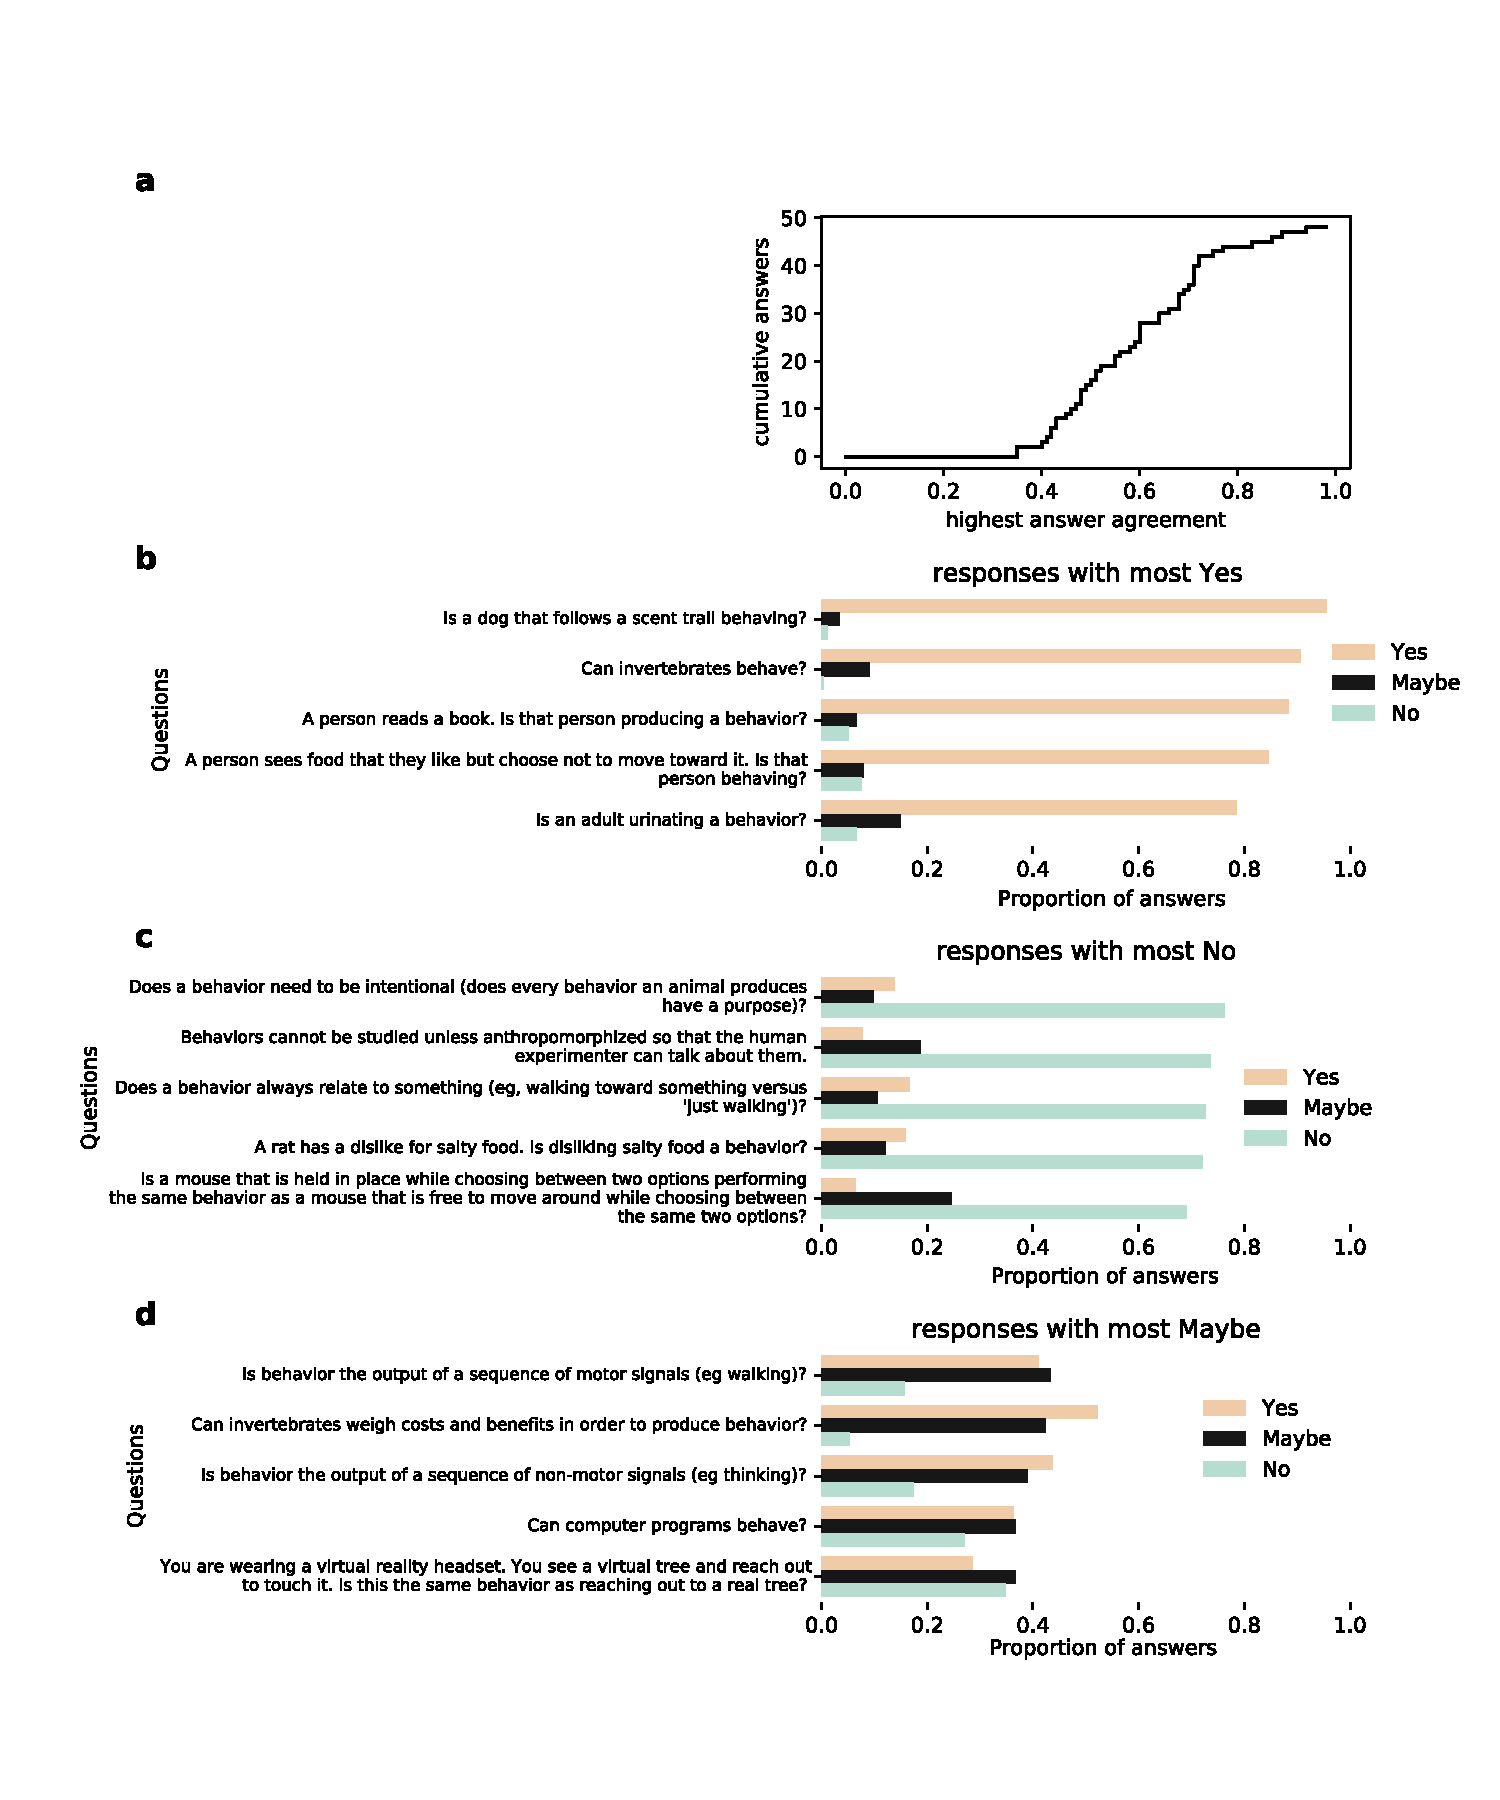
\includegraphics[width=\textwidth]{supp_fig1.pdf}}
\caption{\textbf{General properties of the responses.} \textbf{a}, For each question, the most common answer (eg, 'Yes') was identified and the probability of that response was plotted. Few questions should >80\% consensus.  \textbf{b}, The responses most consistently answered 'Yes'. \textbf{c}, The responses most consistently answered 'No'. \textbf{d}, The responses most consistently answered 'Maybe'.).}
\end{figure}
\newpage

\begin{figure}
\centerline{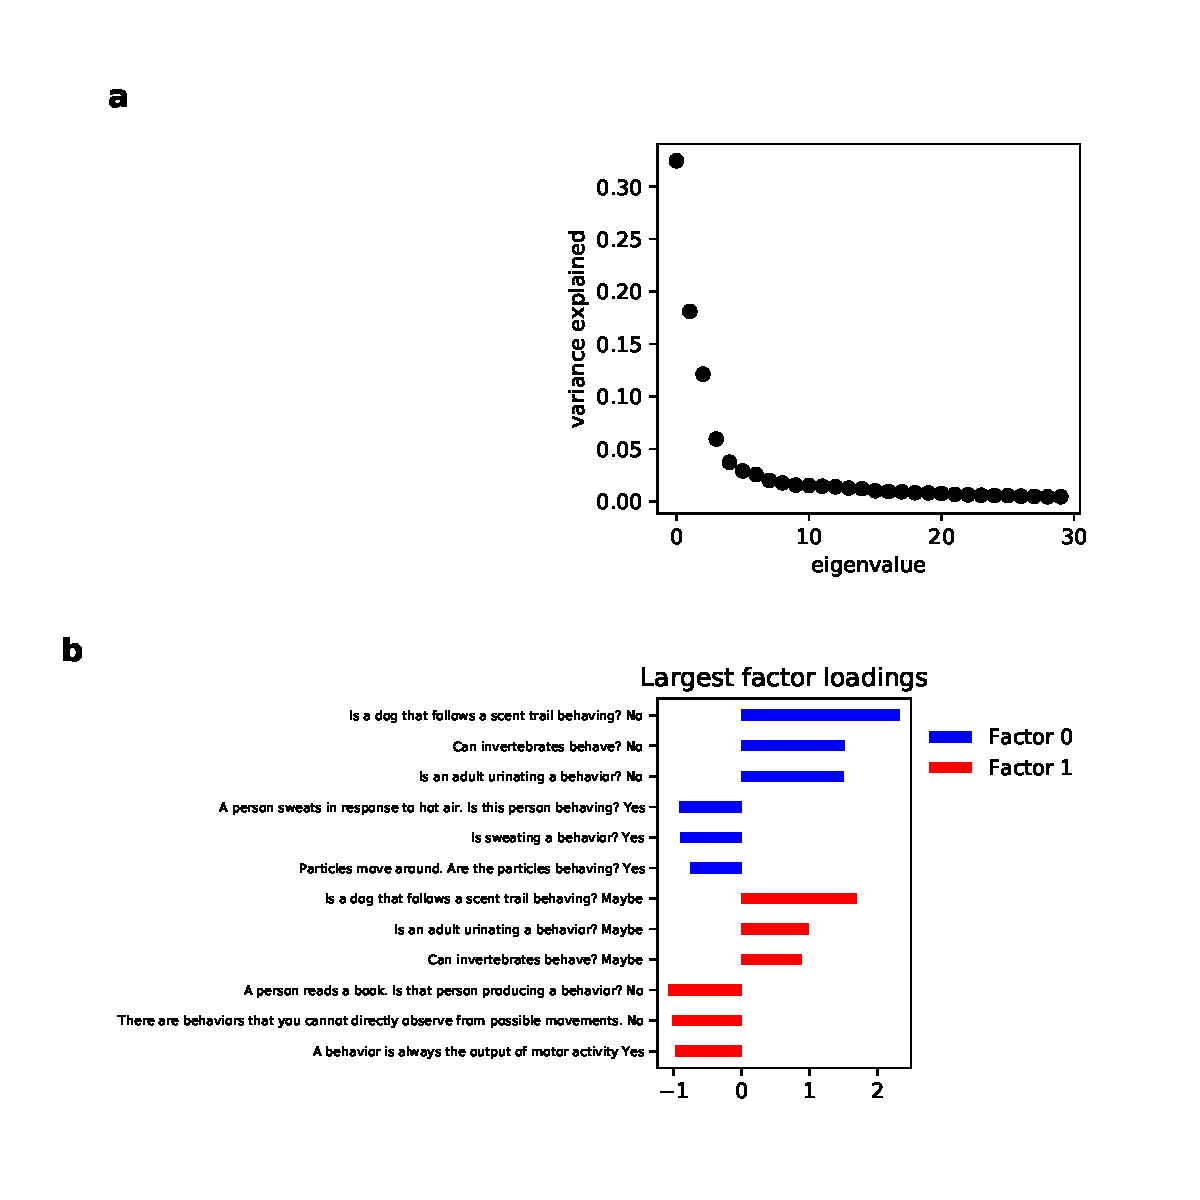
\includegraphics[width=\textwidth]{supp_fig2.pdf}}
\caption{\textbf{Dimensionality reduction.} \textbf{a}, The variance explained for each factor of the MCA space. \textbf{b}, For the two largest dimensions, the questions that showed the three largest positive and three largest negative loadings for the first (blue) and second (red) factors. Because MCA uses one-hot data, loadings are question-answer pairs.}
\end{figure}
\newpage

\begin{figure}
\centerline{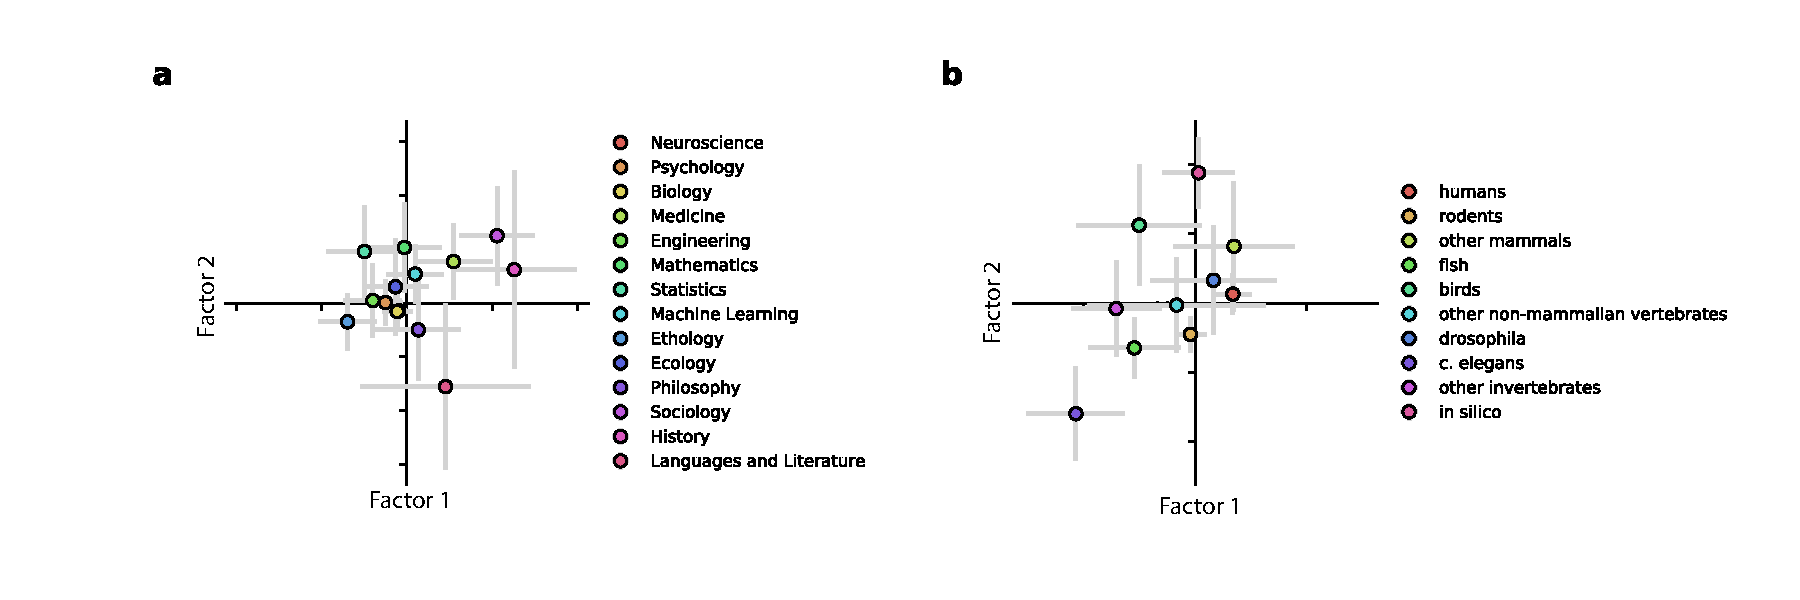
\includegraphics[width=\textwidth]{supp_fig3.pdf}}
\caption{\textbf{Dimensionality reduction in uncombined categories.} The same data as in Figure 1c,e.}
\end{figure}
\newpage

\begin{figure}
\centerline{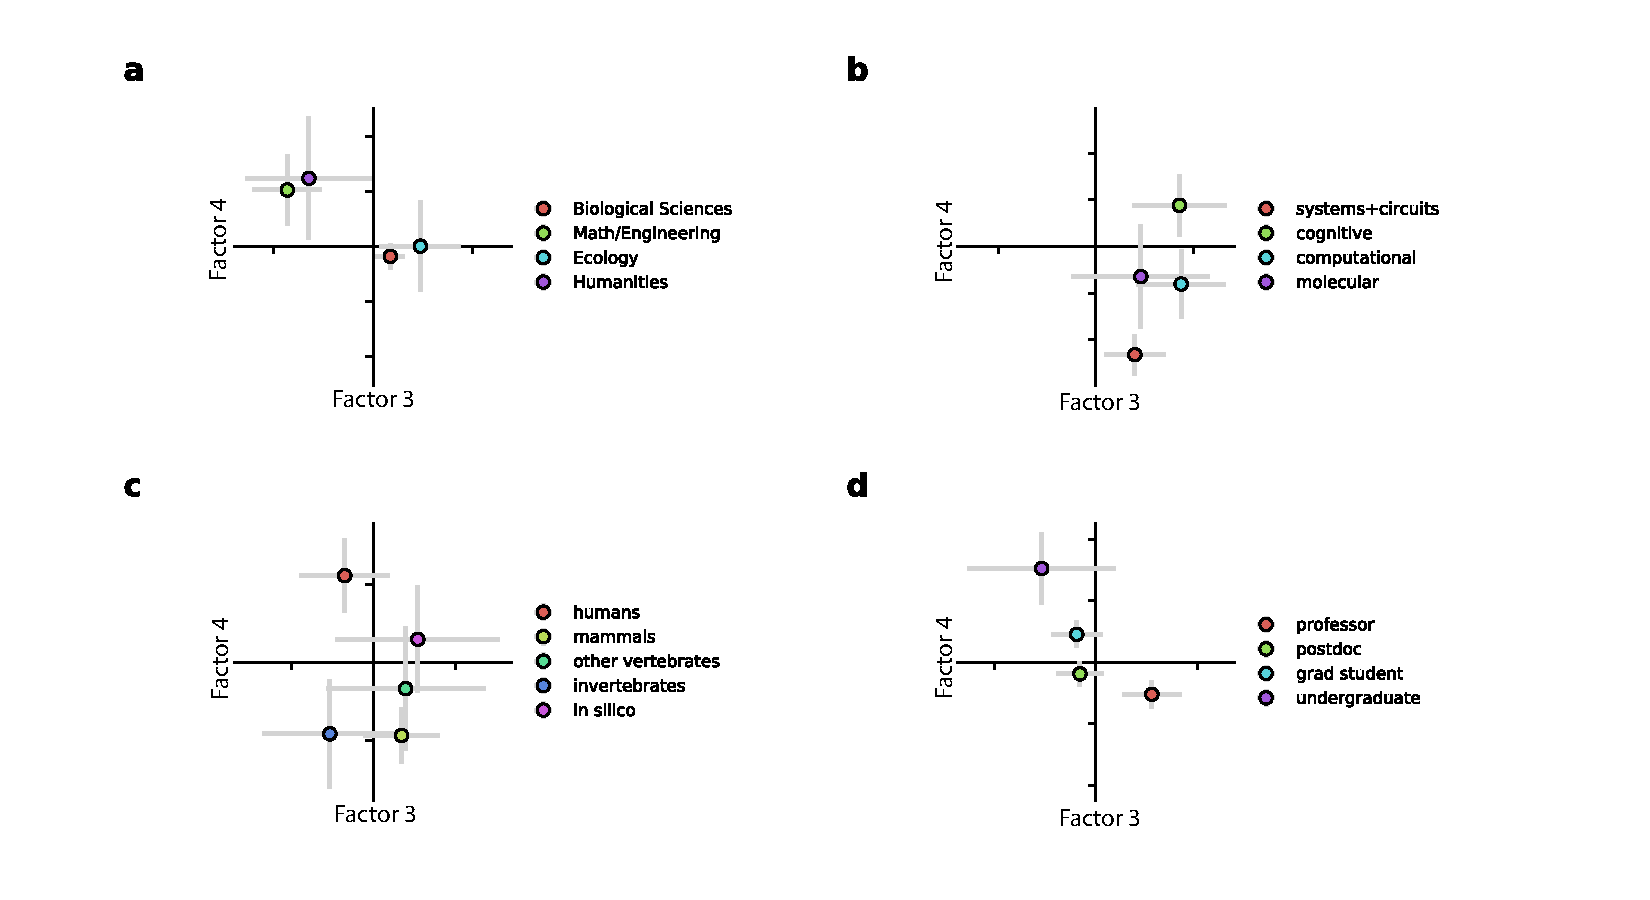
\includegraphics[width=\textwidth]{supp_fig4.pdf}}
\caption{\textbf{Metadata in higher factors.} The same data as in Figure 1c-f, but plotted in the next two largest dimensions.}
\end{figure}
\newpage

\begin{figure}
\centerline{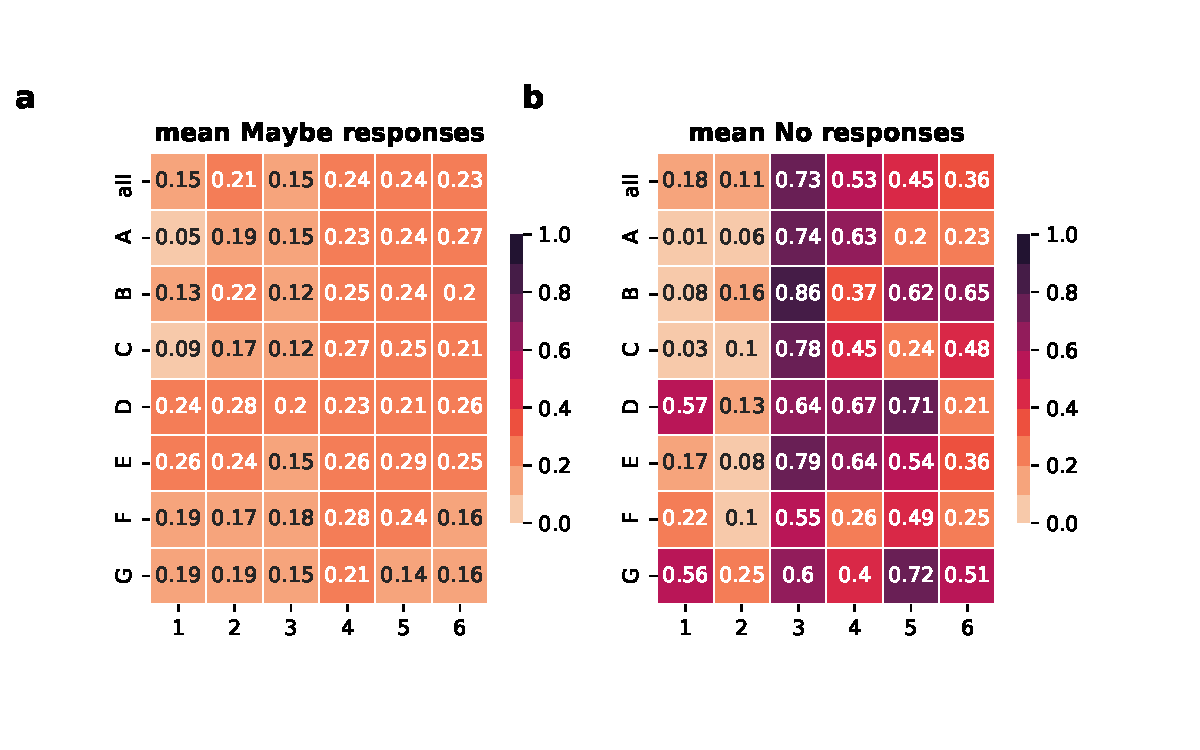
\includegraphics[width=\textwidth]{supp_fig5.pdf}}
\caption{\textbf{Raw response probabilities.} The mean \textbf{a}, Maybe responses and \textbf{b}, No responses for each behavior-type and definition cluster pair. See Figure 3.}
\end{figure}
\newpage

\begin{figure}
\centerline{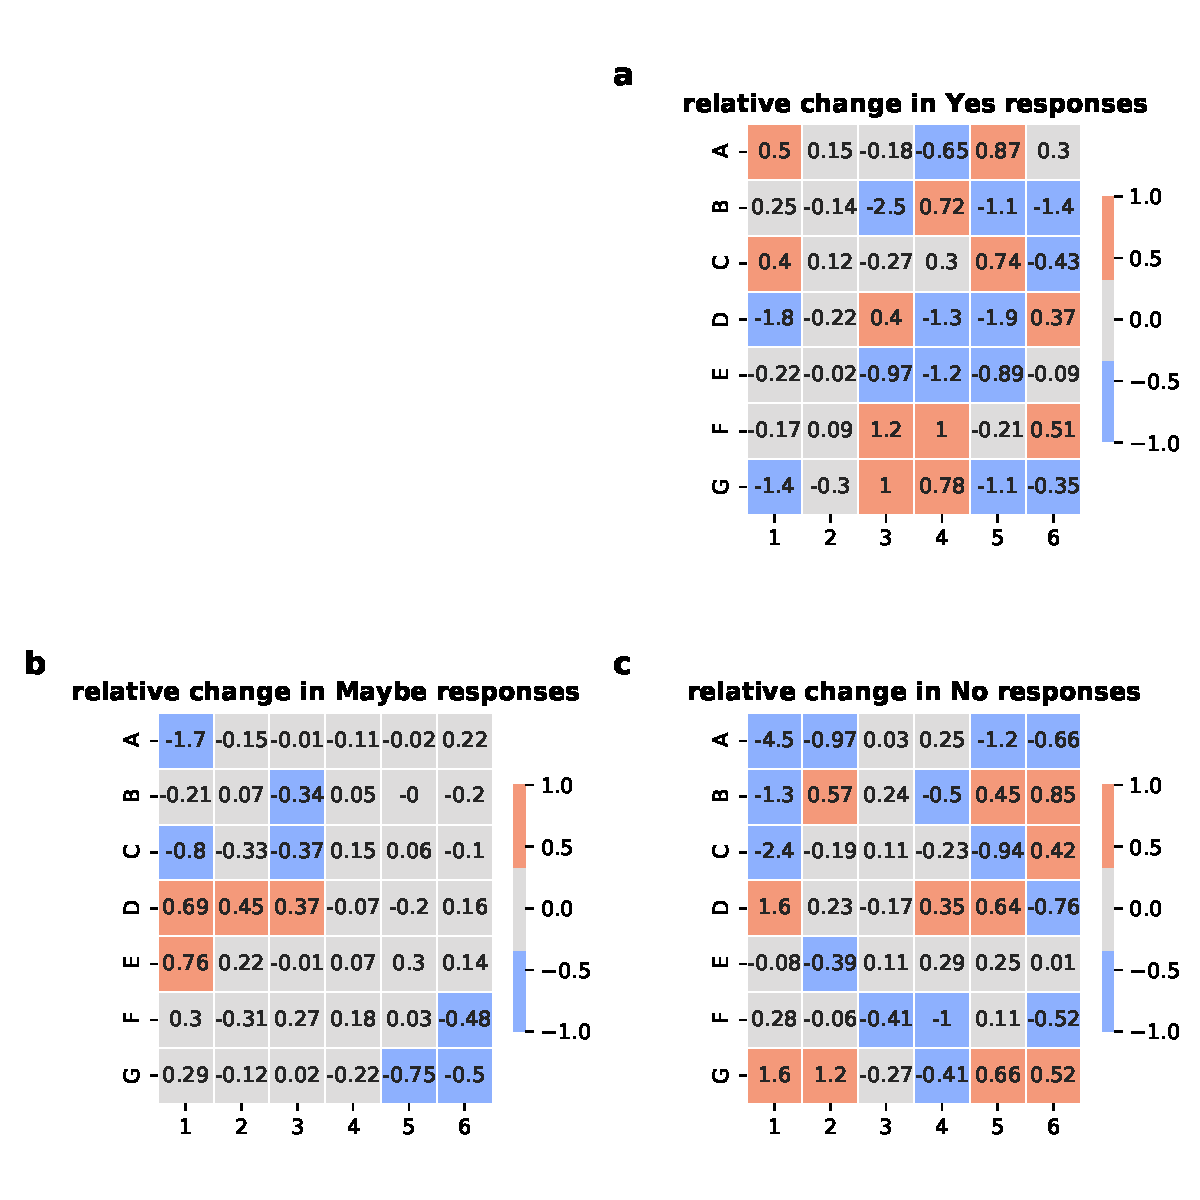
\includegraphics[width=\textwidth]{supp_fig6.pdf}}
\caption{\textbf{Relative changes in responses} The same data as in Supplemental Fig 5, but relative to the mean change across all data.}
\end{figure}
\newpage

\begin{figure}
\centerline{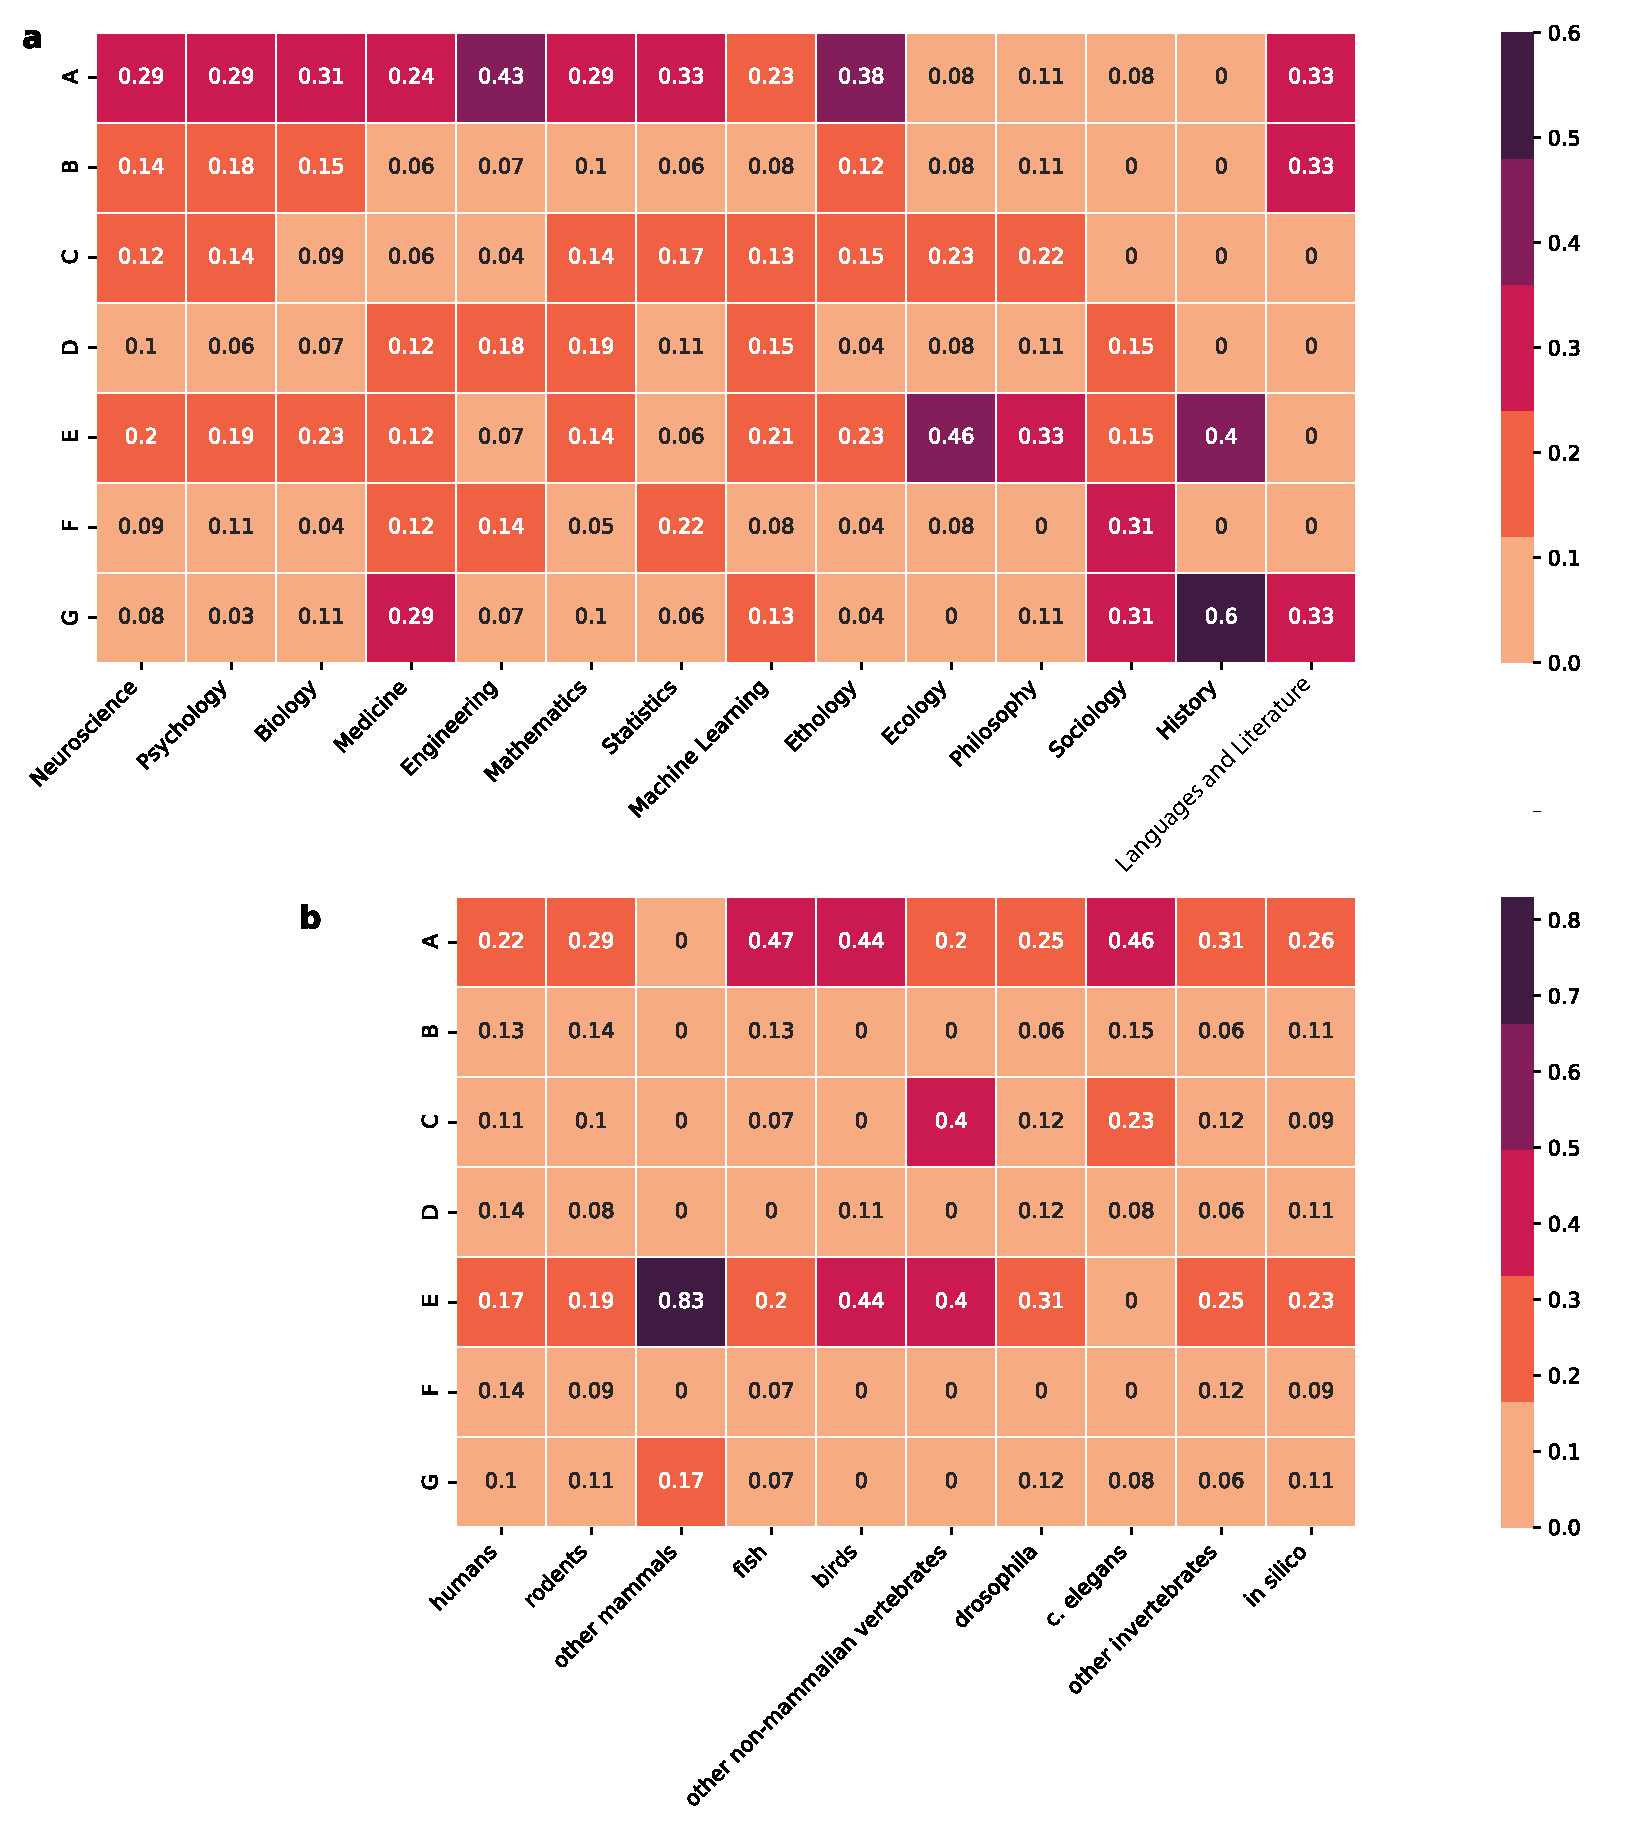
\includegraphics[width=\textwidth]{supp_fig7.pdf}}
\caption{\textbf{Behavioral archetypes in uncompressed categories.} The same data as in Figure 4, replotted by each academic discipline and animal model.}
\end{figure}
\newpage

{\footnotesize \bibliography{behavior.bib}}
% \bibliographystyle{apalike}
\bibliographystyle{plain}
% \printbibliography

\end{document}